\documentclass{article}
\usepackage{tikz}
\usepackage{pgfplots}
\pgfplotsset{compat=1.17}
\usepackage{siunitx}

\begin{document}

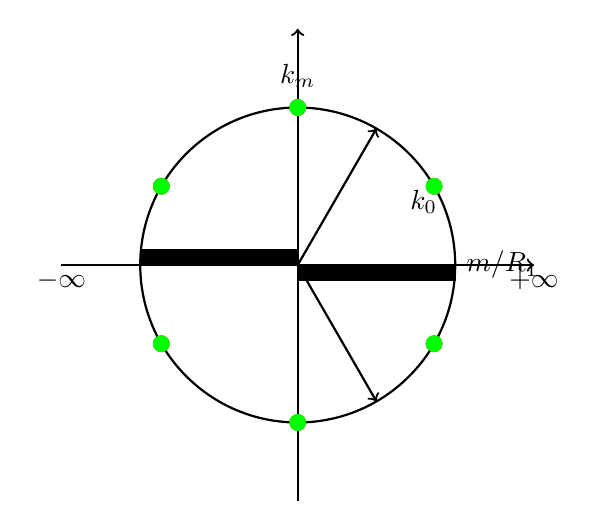
\begin{tikzpicture}[scale=2]
    % Draw the circle
    \draw[thick] (0,0) circle (1);
    
    % Draw the horizontal axis
    \draw[->, thick] (-1.5,0) -- (1.5,0);
    \node at (-1.5,-0.1) {$-\infty$};
    \node at (1.5,-0.1) {$+\infty$};
    
    % Draw the vertical axis
    \draw[->, thick] (0,-1.5) -- (0,1.5);
    
    % Draw the black squares
    \filldraw[black] (-1,0) rectangle (0,0.1);
    \filldraw[black] (1,0) rectangle (0,-0.1);
    
    % Draw the red circles
    \foreach \angle in {30, 90, 150, 210, 270, 330} {
        \filldraw[red] (\angle:1) circle (0.05);
    }
    
    % Draw the green circles
    \foreach \angle in {-30, -90, -150, -210, -270, -330} {
        \filldraw[green] (\angle:1) circle (0.05);
    }
    
    % Draw the labels
    \node at (0,1.2) {$k_m$};
    \node at (0.8,0.4) {$k_0$};
    \node at (1.3,0) {$m/R_1$};
    
    % Draw the arrows
    \draw[->, thick] (0,0) -- (60:1);
    \draw[->, thick] (0,0) -- (-60:1);
    
\end{tikzpicture}

Mode indexing. Red circles correspond to modes travelling radially outwards, and the green circles to modes travelling radially inwards. Positive and negative values of \( m \) correspond to different azimuthal orders. Black squares indicate evanescant modes of which there is a countably infinite number.

\end{document}